\documentclass{article}[11pt]
\usepackage[frenchb,english]{babel}
\usepackage[T1]{fontenc}
\usepackage[utf8]{inputenc}
\usepackage{amsmath,amssymb,latexsym}
\usepackage{times}
\usepackage{float}
\usepackage[left=2cm,right=2cm,top=2cm,bottom=2cm]{geometry}
\frenchbsetup{StandardLists=true} % � inclure si on utilise \usepackage[french]{babel}
\usepackage{enumitem}
\usepackage{fancyhdr}
\usepackage{mathrsfs}
\usepackage{graphicx}
%\usepackage[Algorithme]{algorithm}
%\usepackage{algorithmic}
\usepackage{tikz}
\usepackage{tabularx}
\usetikzlibrary{shapes}
\pagestyle{fancy}
\newcommand{\tr}[1]{{\vphantom{#1}}^{\mathit t}{#1}} 
\renewcommand\headrulewidth{1pt}
\fancyhead[L]{Cours 1�re S}
\fancyhead[R]{Yoann Pietri}
\newcounter{theoremecounter}[subsection]
\usepackage{titlesec}
\setcounter{secnumdepth}{3}% enl�ve la num�rotation apr�s les sections
%\renewcommand\thechapter {\Roman{chapter}}

 \setlength{\parindent}{0pt}

\newcommand{\R}{\mathbb{R}}
\newcommand{\N}{\mathbb{N}}
\newcommand{\Q}{\mathbb{Q}}
\newcommand{\Z}{\mathbb{Z}}
\newcommand{\C}{\mathbb{C}}
\newcommand{\K}{\mathbb{K}}
\newcommand{\eqi}{\Leftrightarrow}
\titleformat{\subsubsection}
   {\normalfont\fontsize{11pt}{13pt}\selectfont\bfseries}% apparence commune au titre et au num�ro
   {\thesubsubsection}% apparence du num�ro
   {1em}% espacement num�ro/texte
   {}% apparence du titre

\tikzstyle{theobox} = [draw=black, very thick,
    rectangle, rounded corners, inner sep=10pt, inner ysep=20pt]
\tikzstyle{theotitle} =[fill=white, text=black,rounded corners,draw=black,very thick]

\fancyhead[L]{Contrôle chapitre 2}

\usepackage{tkz-tab}

\begin{document}
\center
\Large Contrôle de cours (correction)
\flushleft
\center
Fonctions de référence
\flushleft \normalsize
\subsection*{Exercice 1 (R.O.C., temps conseillé : 10 min) : }
On définit la fonction inverse comme $x\mapsto \frac{1}{x}$. Elle est définie sur $\R^*$. On montre que la fonction est décroissante $]0,+\infty[$ : soit $0 \leq a \leq b$ On a $$a\leq b$$ donc $$\frac{a}{b}\leq 1$$
$$\frac{1}{a}\frac{a}{b} \leq \frac{1}{a}$$ finalement $$\frac{1}{b} \leq \frac{1}{a}$$ On montre maintenant que la fonction est croissante $]-\infty,0[$ : soit $b\leq a\leq 0$ On a $$b\leq a$$ donc $$\frac{b}{a}\geq 1$$
$$\frac{1}{b}\frac{b}{a} \leq \frac{1}{b}$$ finalement $$\frac{1}{a} \leq \frac{1}{b}$$ 
\center
\begin{tikzpicture}[scale=0.5]
\draw[very thin, step=0.5,color=gray!60](-5,-5) grid(5,5); 
\draw[thin,color=gray] (-5,-5) grid(5,5);
\draw [thick, ->] (-5,0)--(5,0) node [below left] {$x$ }; 
\draw [thick, ->] (0,-5)--(0,5) node [below left] {$y$};
\draw [domain=-5:-0.2,color=red,samples=100] plot (\x, 1/\x);
\draw [domain=0.2:5,color=red,samples=100] plot (\x, 1/\x);
\draw (1,0) node [below] {1};
\draw (0,1) node [left] {1};
\draw (0,0) node [below left] {0};
\draw [thick,dashed] (-1,-1) -- (1,1);
\end{tikzpicture}\newline
\flushleft
\subsection*{Exercice 2 (Etude d'une fonction, temps conseillé : 15-18 min) : }
\begin{enumerate}
\item On calcule le discriminant 
$$\Delta = 12^2-4\times2\times16 = 16$$
$\Delta > 0$ donc le trinôme admet deux racines réelles distinctes qui sont 
$$x_1 = \frac{12 - \sqrt{16}}{2\times2} = \frac{12 - 4}{2\times2} = 2$$
$$\boxed{x_1 = 2}$$
$$x_2 = \frac{12 + \sqrt{16}}{2\times2} = \frac{12 + 4}{2\times2} = 4$$
$$\boxed{x_2 = 4}$$
\item Le coefficient dominant étant positif
\begin{tikzpicture}
   \tkzTabInit{$x$ / 1 , $g(x)$ / 1}{$-\infty$,$2$,$4$, $+\infty$}
   \tkzTabLine{, +,z,-,z, +,}
\end{tikzpicture}
\item On déduit le domaine de définition de $x\mapsto \sqrt{g(x)}$ est $]-\infty,2] \cup [4,+\infty[$ qui s'annule en $x=2$ et $x=4$ donc le domaine de définition de $f$ est $]-\infty,2[ \cup ]4,+\infty[$
\item La racine garde le sens de variation donc $x\mapsto \sqrt{g(x)}$ est décroissante sur $]-\infty,2]$ et croissante sur $[4,+\infty[$
\item La fonction inverse inverse le sens de variation (lol). Ainsi $f$ est croissante sur $]-\infty,2[$ et décroissante sur $]4,+\infty[$
\item On a
$$f(-1) = \frac{1}{\sqrt{2(-1)^2 +12+16}} = \frac{1}{\sqrt{30}}$$
$$\boxed{f(-1) = \frac{1}{\sqrt{30}}}$$
$$f(5) = \frac{1}{\sqrt{2(5)^2 -12\times 5+16}} = \frac{1}{\sqrt{6}}$$
$$\boxed{f(5) = \frac{1}{\sqrt{6}}}$$
\item Voici la représentation graphique de $f$ \newline

\center
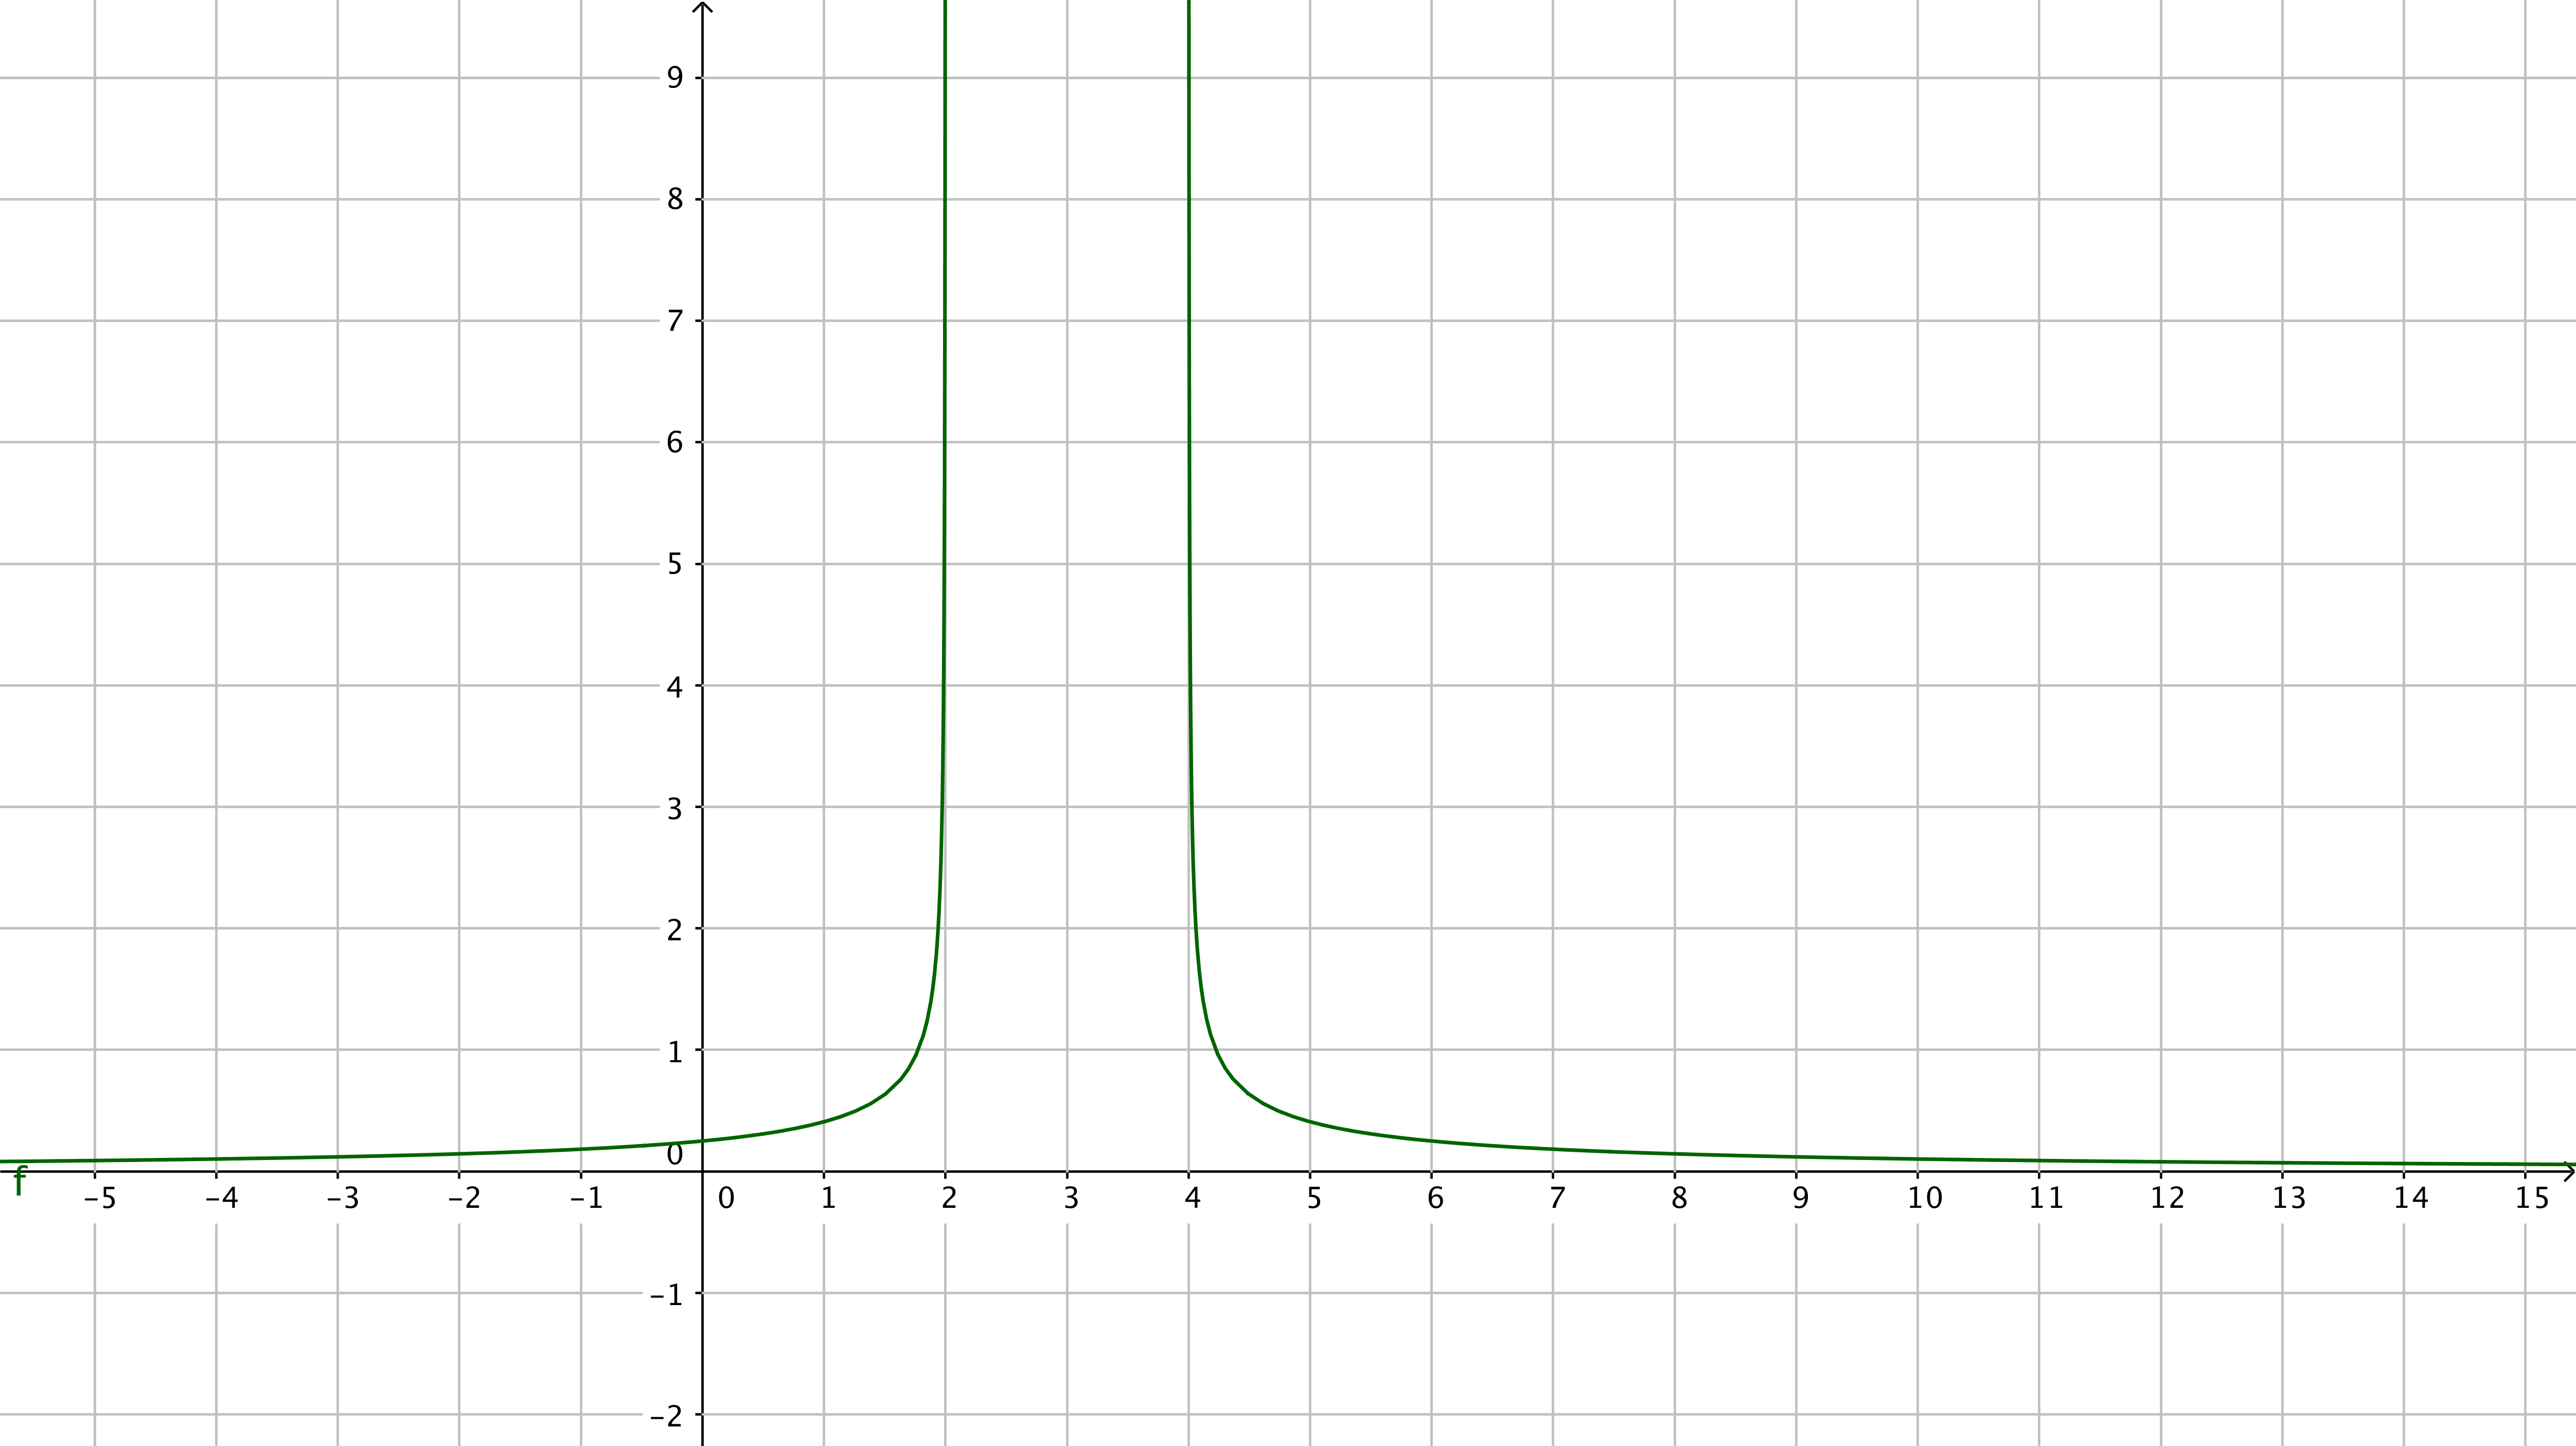
\includegraphics[scale=0.7]{chap2_corr_ill1.png}
\flushleft
\end{enumerate}
\subsection*{Exercice 3 (Valeur absolue, temps conseillé : 10 min) : }
\begin{enumerate}
\item On appelle valeur absolue la fonction définie par 
$$|x| = \left\{\begin{array}{l}x \text{ si } x \geq 0 \\ -x \text{ si } x\leq 0\end{array}\right.$$
\item On étudie tous les cas \newline

\begin{tabularx}{\linewidth}{| X | X | X | X |}
\hline
$a \geq 0; b \geq 0$ & $a \leq 0; b \geq 0$ & $a \geq 0; b \leq 0$ & $a \leq 0; b \leq 0$ \\ \hline
Alors $$|a| = a$$ $$|b| = b$$ De plus $$ab \geq 0$$ donc $$|ab| = ab$$ OK & Alors $$|a| = -a$$ $$|b| = b$$ De plus $$ab \leq 0$$ donc $$|ab| = -ab$$ OK & Alors $$|a| = a$$ $$|b| = -b$$ De plus $$ab \leq 0$$ donc $$|ab| = -ab$$ OK & Alors $$|a| = -a$$ $$|b| = -b$$ De plus $$ab \geq 0$$ donc $$|ab| = ab$$ OK\\ \hline
\end{tabularx}
\item On remarque une identité remarquable : $h(x) = (x-2)^2$. Donc pour tout $x\in \R$, $h(x) \geq 0$ donc pour tout $x\in \R, |h(x)| = h(x)$
\end{enumerate}
\subsection*{Exercice 4 (Intersection de deux droites, temps conseillé : 17-20 min) : }
\begin{enumerate}
\item Pas de point en commun : droite parallèle non confondue (exemple : $d_1:x=1$ et $d_2:x=2$), un point en commun : droites non parallèles (exemple : $d_1:x=0$, $d_2:y=0$) et infinité de points en commun : droites confondues (exemple :$d_1:x+y=1$, $d_2:x+y=1$)
\item Si $(x,y)$ est un point d'intersection, alors 
$$y = ax+b$$ et $$y = cx+d$$ donc $$y-y = ax+b - (cx+d)$$ donc $$0 = ax - cx + b-d$$ donc 
$$\boxed{(a-c) x = d-b}$$
\item On suppose tout d'abord $a-c = 0$. L'équation devient alors $d-b = 0$ \newline
Si $d =b $ alors $f=g$ et il y a une infinité de point en commun puisque les droites sont confondues\newline
Si $d \neq b$ alors il ne peut y avoir de point en commun donc les droites sont parallèles non confondues
\item On revient à l'équation $$(a-c) x = d-b$$ vu que $a-c\neq 0$, on divise par $a-c$ et on trouve $$\boxed{x = \frac{d-b}{a-c}}$$ On réinjecte $x$ dans $y=ax+b$ pour trouver $y$ : $$y = a\frac{d-b}{a-c} +b$$ $$ y=\frac{ad-ba +ba -bc}{a-c}$$ $$\boxed{y=\frac{ad-bc}{a-c}}$$ On déduit que bien que le point d'intersection est  $$\left(\frac{d-b}{a-c} ,\frac{ad-bc}{a-c}\right)$$
\end{enumerate}
$$\star \star \star$$
\center
FIN DU SUJET
\end{document}